\documentclass[a4paper, 11pt, titlepage]{article}
\usepackage{times}
\usepackage[czech]{babel}
\usepackage[utf8]{inputenc}
\usepackage[ddmmyyyy]{datetime}
\renewcommand{\dateseparator}{--}
\usepackage[left=2cm,text={17cm, 24cm},top=3cm]{geometry}
\usepackage{multirow}
\usepackage{graphicx}
\usepackage{pdfpages}
\usepackage{svg}
\usepackage{textcomp}
\usepackage{multicol}
\usepackage{vwcol}
\usepackage{bm}
\usepackage{amsmath}
\usepackage{graphicx}
\usepackage{hhline}
\usepackage{float}
\usepackage{fancyvrb}
\restylefloat{table}
\graphicspath{ {images/} }
\renewcommand{\dateseparator}{.}
\setlength{\parskip}{0.5em}
\bibliographystyle{czplain}


\begin{document}

\begin{titlepage}
	\begin{center}
		{\Huge		
			\textsc{Vysoké učení technické v~Brně}}\\
			\medskip
		{\huge
			\textsc{Fakulta informačních technologií}}\\
		
\includegraphics{logo.pdf}\\
			\vspace{\stretch{0.2}}
		{\Huge
			Praktická úloha řešená sítí RCE}\\
		\bigskip
		{\LARGE
			Projekt do předmětu SFC, 2019/2020}\\
		\medskip
		\vspace{\stretch{0.618}}	
	\end{center}
	{\Large Tomáš Blažek (xblaze31) \hfill \today}
\end{titlepage}

\section{Úvod}
Cílem bylo vytvořit aplikaci, která implementuje funkci neuronové sítě RCE (Restricted Coulomb Energy) a následně vhodně zvolit praktickou úlohu, která by byla neuronovou sítí RCE řešena. Tím je myšlena úloha, u které by byla možná jednoduchá validace výsledků odezvy neuronové sítě a případně nenáročné zadávání vstupu. Primárním cílem je ukázat především funkci a vlastnosti neuronové sítě této architektury.

\section{Architektura neuronové sítě RCE}
Jedná se o dvouvrstvou neuronovou síť s proměnnou topologií. První vrstva, která se nazývá skrytá, obsahuje radiální bázovou funkci a skokovou aktivační funkci. Druhá vrstva, která je vrstvou výstupní, má odezvu logické funkce OR. Výpočet vnitřího potenciálu neuronů skryté vrstvy $u_k$ je podle vzorce \ref{eq:base_rce}, kterým se jinak řečeno spočítá vzdálenost mezi vektorem vah $\vec{w_k}$ (střed hyperkoule) a vstupním vektorem $\vec{i}$.\cite{rceZboril}
\begin{equation}
\label{eq:base_rce}
u_k = \sqrt{\sum_{i=1}^{n}(i_i - w_{ki})^2}
\end{equation}
Aktivační funkce skryté vrstvy je dána vzorcem \ref{eq:activation_rce}. Jedná se o skokovou funkci a nabývá buď hodnotu 1 anebo hodnotu 0. To podle toho, zda-li je vzorek uvnitř hyperkoule daného neuronu $k$ (tj. 1), anebo se nachází mimo ni (tj. 0). Velikost hyperkoule je definována poloměrem $r_k$, pro každý neuron.
\begin{equation}
\label{eq:activation_rce}
y_k = \left\{
  \begin{array}{lr}
    1 & : u_k\le r_k\\
    0 & : u_k > r_k 
  \end{array}
\right.
\end{equation}
Neuronové síťě s radiální bázovou funkcí, jako jsou právě neuronové síťě RCE, jsou vhodné například ke klasifikaci a funkční aproximaci v $n$-dimensionálním prostoru.

\begin{figure}[H]
    \centering
    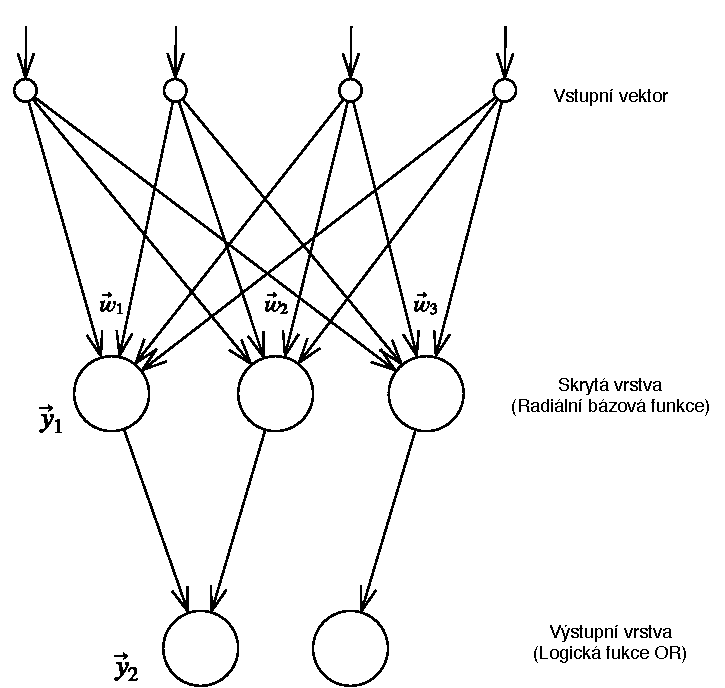
\includegraphics[scale=0.8]{rce.pdf}
    \caption{Architektura RCE neuronové sítě}
    \label{fig:rce}
\end{figure}

\section{Řešená úloha}
\label{resena_uloha}
Jako praktická úloha, která má být řešena neuronovou síťí RCE, byla zvolena úloha balančních vah. Byla zvolena především z důvodu toho, že výsledky poskytnuté neuronovou sítí je možné snadno ověřit. 
\begin{figure}[H]
    \centering
    
\includegraphics[scale=0.75]{balance-scale.pdf}
    \caption{Ilustrační obrázek balančních vah\cite{Dua2019}}
    \label{fig:balance-scale}
\end{figure}
Úloha spočívá v tom, že máme k dispozici balanční váhy se dvěma miskam, jak je uvedeno na obrázku \ref{fig:balance-scale}. Do obou misek je možné umístit závaží o určité hmotnosti a vzdálenosti od středu váhy. Množina dat, na níž je síť trénovaná\footnote{Kokrétní dataset je možné získat na adrese http://mlr.cs.umass.edu/ml/datasets/Balance+Scale}, byla získána z Machine Learning Repository\cite{Dua2019} a obsahuje vektory ve tvaru:
$$\texttt{Class-Name, Left-Weight, Left-Distance, Right-Weight, Right-Distance}$$
Jednotlivé atributy mohou nabývat různých hodnot:
\begin{itemize}
	\item \textbf{Class-Name}: Označuje náklon balanční váhy a může nabývat tří hodnot. (Left, Balanced, Right)
	\item \textbf{Left-Weight}: Váha, která je umístěna na levou část váhy. Trénovací množina obsahuje následující hodnoty. (1, 2, 3, 4, 5)
	\item \textbf{Left-Distance}: Vzdálenost od středu váhy, na které je položeno závaží na levou misku. Trénovací množina obsahuje následující hodnoty. (1, 2, 3, 4, 5)
	\item \textbf{Right-Weight}: Váha, která je umístěna na pravou část váhy. Trénovací množina obsahuje následující hodnoty. (1, 2, 3, 4, 5)
	\item \textbf{Right-Distance}: Vzdálenost od středu váhy, na které je položeno závaží na pravou misku. Trénovací množina obsahuje následující hodnoty. (1, 2, 3, 4, 5)
\end{itemize}



\section{Implementace}
Aplikace je rozložena do několika balíčků (packages) rozčleněných podle funkční logiky. Do hlavního balíčku spadají třídy \texttt{Main} a \texttt{Arguments}, které se starají o zpracování vstupních argumentů a hlavního chodu aplikace. Dále jsou to balíčky \texttt{io} a \texttt{net}.
\begin{figure}[H]
    \centering
    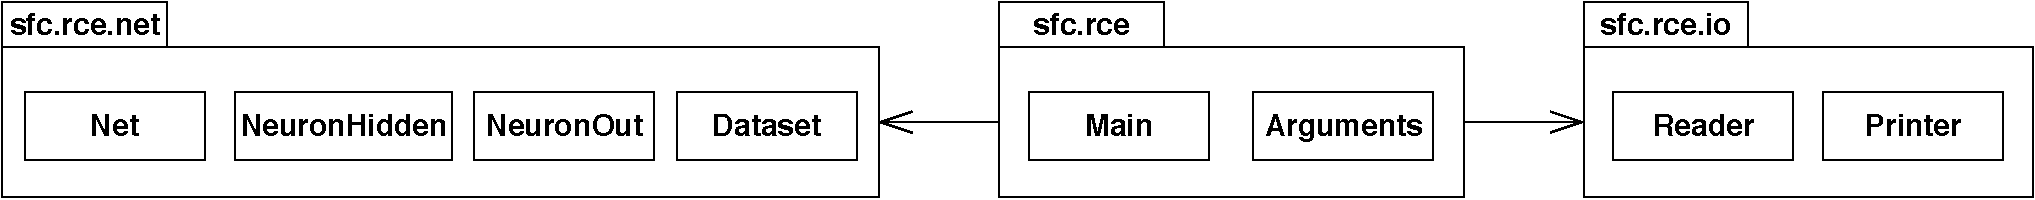
\includegraphics[scale=0.5]{package_diagram_flat.pdf}
    \caption{Diagram balíčků aplikace}
    \label{fig:package_diagram}
\end{figure}
\subsection{Balíček net}
Tento balíček obsahuje čtyři třídy, které implementují algoritmus RCE neuronové sítě. Základní třídou tohoto balíčku je třída \texttt{Net}, která obsahuje fukce pro inicializaci sítě, trénování sítě, klasifikaci apod. Dále obsahuje třídy \texttt{NeuronHidden} a \texttt{NeuronOut}, které slouží k ukládání jednotlivých vzahů mezi neurony v síti. Jako poslední v tomto balíčku je třída \texttt{Dataset}, jejímž úkolem je práce s množinou vektorů, s níž neuronová síť pracuje.

\subsection{Balíček io}
Obsahuje třídy \texttt{Reader} a \texttt{Printer}, které implementují vstupní a výstupní operace. Třída \texttt{Reader} načítá vstupní data v podobně řetězce a převádí je do vnitřní implementace v podobně datasetu (třída \texttt{Dataset}). Dále se tato třída stará o komunikaci s uživatelem. Třída \texttt{Printer} slouží pro výpis dat uživateli ve formátované podobě.

\subsection{Implementační technologie}
Technologie použité pro implementaci byly zvoleny následující. Programovací jazyk Java~(verze 1.8) a nástroj Apache Ant sloužicí pro kompilaci zdrojových kódú, sestavení výchozí operace a vygenerování programové dokumentace.

\section{Manuál}
Aplikaci je nutno před použitím přeložit k vytvoření spustitelného archivu jar. Následující podkapitoly popisují postupy pro překlad, spuštění a ovládání programu.

\subsection{Překlad}
V kořenovém adresaři je soubor \texttt{build.xml}, který obsahuje informace potřebné k překladu pomocí nástroje Apache Ant. Stačí tedy v tomto adresáři použít příkaz:
$$\texttt{ant compile}$$
Ten provede překlad zdrojových kódů. Výsledky překladu jsou následně uloženy do složky adresáře \texttt{build}. Spustitelná aplikace je vygenerována v kořenovém adresáři jako jar soubor s názvem \texttt{sfc-rce.jar}. Jako další akci provede tento příkaz vygenerování programové dokumentace do adresáře \texttt{doc/program}.\cite{antApache}

\subsection{Použití}
Aplikace se spustí pomocí příkazu příkazu:
$$\texttt{java -jar sfc-rce.jar}$$
Následně se bude aplikace ptát na vstupní vzorek v podobně jednoduchých dotazů. Nicméně v tomto momentě je v aplikaci nenatrénovaná neuronová síť. Tím pádem budou všechny odpovědi sítě ve tvaru \uv{Unkwown}. Pro spuštění tréninku sítě je nutné použít přepínač \texttt{-t <soubor\_s\_trénovací\_množinou>}.

\subsubsection*{Popis přepínačů}
Při spuštění aplikace je možno využít přepínačů a nakonfigurovat si tak neuronovou síť před použitím podle potřeby.
\begin{itemize}
\item \texttt{-t <soubor\_s\_trénovací\_množinou>}\\
	  Tento přepínač umožňuje zvolit soubor s trénovací množinou, kterou má být síť natrénována. Formát obsahu toho souboru by měl mít strukturu takovou, že na každé řádku se vyskytuje jeden vektor (vzorek) trénovací množiny a vektor je ve formátu sekvence čísel oddělených čárkou. První hodnota v tomto sloupci nemusí být číslo, jelikož označuje cílovou třídu daného vzorku.
\item \texttt{-v <soubor\_s\_validační\_množinou>}\\
      Podobně jako předchozí přepínač nastavuje nastavuje soubor. Tentokrát je to ale soubor s validační množinou. Při zadání tohoto přepínače neuronová síť klasifikuje všechny vzorky v souboru, vypíše na výstup výsledky této klasifikace a aplikace se ukončí.
\item \texttt{-R <maximální\_velikost\_hyperkoule>}\\
      Aplikace umožňuje nakonfigurovat maximální velikost hyperkoulí při vytváření/učení neuronové sítě.
\item \texttt{-r <zmenšovací\_poměr\_hyperkoule>}\\
	  Aplikace umožňuje nakonfigurovat poměr jakým se budou hyperkoule zmenšovat při trénování neuronové sítě. Jeho hodnota by se měla pohybovat v intervalu $(0,1)$.
\end{itemize}

\subsection{Závěr}
Neuronová síť dosahovala úspěšnosti klasifikace kolem 80\,\%. Síti byly předloženy dvě množiny, jedna určená na natrénování sítě a druhá pro validaci odezvy. Ty byly vytvořeny z již zmíňěné množiny dat z kapitoly \ref{resena_uloha}. Vzorky byly náhodně zamíchány a prvních 525 vzorků bylo zvoleno jako tréninková množina a zbylých 100 jako validační množina. Úspěšnost klasifikace závisela z velké části na zvolených parametrech síťě, a to na maximální velikosti hyperkoule a zmenšovacím poměru.

\newpage
\raggedright
\bibliography{zdroje}

\end{document}